\documentclass[a4paper,11pt]{article}

\usepackage{appendixnumberbeamer}
\usepackage{booktabs}
\usepackage[scale=2]{ccicons}
\usepackage{pgfplots}
\usepackage{xspace}
\usepackage{bookmark}
\usepackage{amssymb}
\usepackage{mathtools}
\usepackage[normalem]{ulem}
\usepackage[T1]{fontenc}
\usepackage[sfdefault,book]{FiraSans}
\usepackage{FiraMono}
\usepackage{fontawesome}
\usepackage{listings}
\usepackage{hyperref}
\usepackage[10pt]{moresize}

\renewcommand*\familydefault{\ttdefault}

\renewcommand{\thefootnote}{\fnsymbol{footnote}}
\renewcommand{\MintedPygmentize}{/home/thiago/.local/bin/pygmentize}

\definecolor{light-gray}{gray}{0.95}
\renewcommand\lstlistingname{Código}
\DeclareCaptionFormat{listing} {
  \parbox{\textwidth}{\hspace{-0.2cm}#1#2#3}
}
\DeclareCaptionFont{black}{\color{black}}
\captionsetup[lstlisting]{
  format=listing,
  labelfont=black,
  textfont=black,
  singlelinecheck=true,
  margin=0pt,
  font={tt,footnotesize,bf}
}

\lstset{
  basicstyle=\footnotesize\ttfamily,
  escapeinside={\%*}{*)},
  mathescape=true,
  showspaces=false,
  showtabs=false,
  showstringspaces=false,%
  % backgroundcolor=\color{light-gray},
  rulesepcolor=\color{black},
  frame=shadowbox,
  literate=
  {á}{{\'a}}1 {é}{{\'e}}1 {í}{{\'i}}1 {ó}{{\'o}}1 {ú}{{\'u}}1
  {Á}{{\'A}}1 {É}{{\'E}}1 {Í}{{\'I}}1 {Ó}{{\'O}}1 {Ú}{{\'U}}1
  {à}{{\`a}}1 {è}{{\`e}}1 {ì}{{\`i}}1 {ò}{{\`o}}1 {ù}{{\`u}}1
  {À}{{\`A}}1 {È}{{\'E}}1 {Ì}{{\`I}}1 {Ò}{{\`O}}1 {Ù}{{\`U}}1
  {ä}{{\"a}}1 {ë}{{\"e}}1 {ï}{{\"i}}1 {ö}{{\"o}}1 {ü}{{\"u}}1
  {Ä}{{\"A}}1 {Ë}{{\"E}}1 {Ï}{{\"I}}1 {Ö}{{\"O}}1 {Ü}{{\"U}}1
  {â}{{\^a}}1 {ê}{{\^e}}1 {î}{{\^i}}1 {ô}{{\^o}}1 {û}{{\^u}}1
  {Â}{{\^A}}1 {Ê}{{\^E}}1 {Î}{{\^I}}1 {Ô}{{\^O}}1 {Û}{{\^U}}1
  {Ã}{{\~A}}1 {ã}{{\~a}}1 {Õ}{{\~O}}1 {õ}{{\~o}}1
  {œ}{{\oe}}1 {Œ}{{\OE}}1 {æ}{{\ae}}1 {Æ}{{\AE}}1 {ß}{{\ss}}1
  {ű}{{\H{u}}}1 {Ű}{{\H{U}}}1 {ő}{{\H{o}}}1 {Ő}{{\H{O}}}1
  {ç}{{\c c}}1 {Ç}{{\c C}}1 {ø}{{\o}}1 {å}{{\r a}}1 {Å}{{\r A}}1
  {€}{{\euro}}1 {£}{{\pounds}}1 {«}{{\guillemotleft}}1
  {»}{{\guillemotright}}1 {ñ}{{\~n}}1 {Ñ}{{\~N}}1 {¿}{{?`}}1
}

\setminted{
  fontsize=\footnotesize,
  style=xcode,
  frame=single,
  framesep=3\fboxsep,
  labelposition=topline,
}


\title{Análise e Projeto de Algoritmos -- Exercícios 02 (Grafos)}
\author{Prof. Thiago Cavalcante}
\date{}

\begin{document}

\pagenumbering{gobble}
\maketitle

\sloppy
\raggedright

\setlength{\leftmargini}{0pt}
\begin{enumerate}
  % BFS
  \item Obtenha os valores de distância e parentesco para a execução do BFS no grafo dirigido a seguir, usando o vértice 3 como inicial.

  \begin{center}
    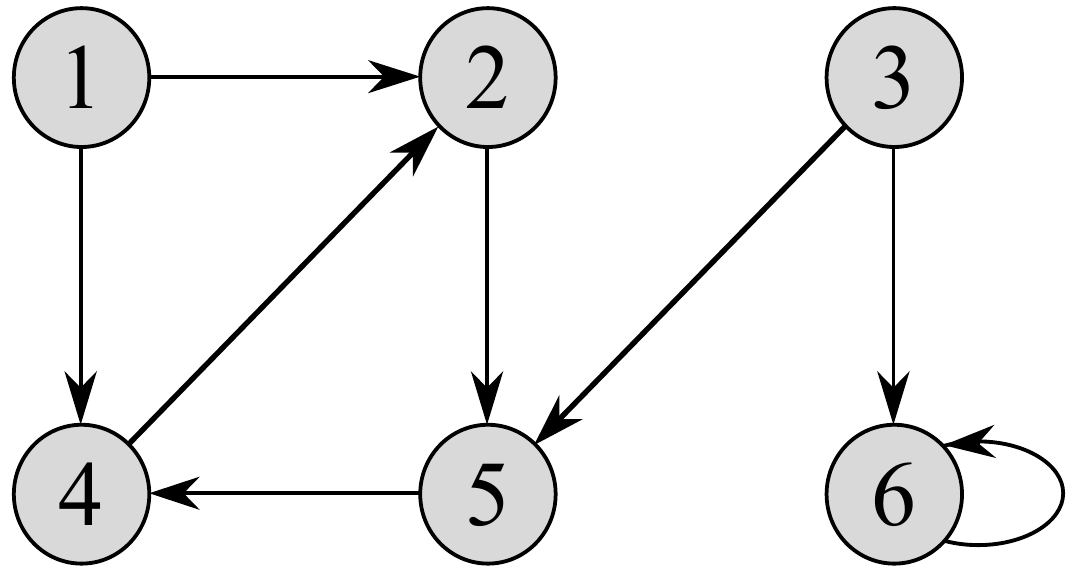
\includegraphics[width=.5\textwidth]{graph2.png}
  \end{center}

  \item Obtenha os valores de distância e parentesco para a execução do BFS no grafo não-dirigido a seguir, usando o vértice u como inicial.

  \begin{center}
    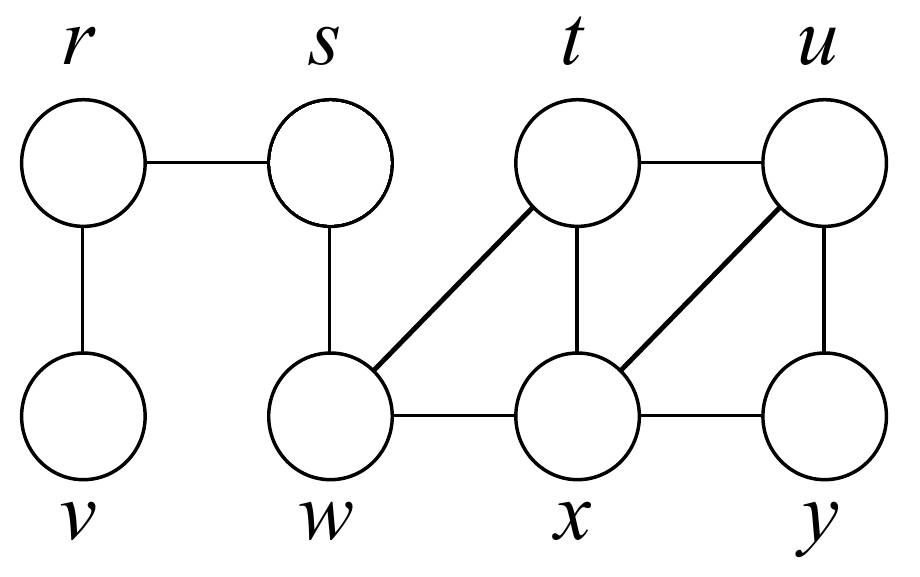
\includegraphics[width=.5\textwidth]{graph3.png}
  \end{center}

  % ORDENAÇÃO TOPOLÓGICA
  \item Faça a ordenação topológica do grafo a seguir
  \bigskip

  \begin{center}
    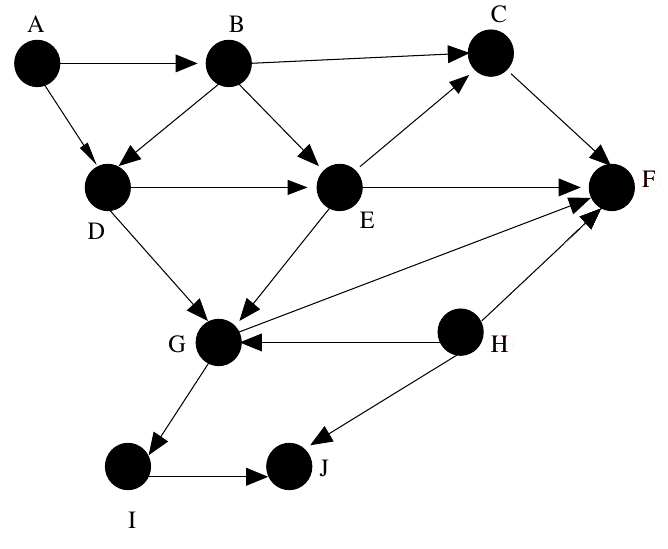
\includegraphics[width=.5\textwidth]{graph1.png}
  \end{center}
\end{enumerate}
\end{document}
